
 \title{
\includegraphics[height=0.08\textheight] {logo-dipartimento.png} \\ \LARGE Progetto Ingegneria del Software \\ \normalsize Model Based Software Engineering\\ \small A.A. 2020-2021} %ATTENZIONE il  file  “logo-dipartimento.png” non è presente all’interno della directory /Figure per motivi legati alla proprietà e diffisione del logo, se si vuole compilare il file cancellare l’inserimetno dell’immagine.

\author{Lorenzo Camilli}
\date {}	

\documentclass[a4paper,14pt,]{report}
\usepackage{booktabs}
\usepackage[T1]{fontenc} 
\usepackage[utf8]{inputenc}
\usepackage[italian]{babel} 
\usepackage{geometry} 
%\geometry{a4paper,top=3cm,bottom=3cm, left=3cm,right=3cm, heightrounded,bindingoffset=5mm}		
\pagestyle{plain}		
\usepackage{graphicx}	
\usepackage{hyperref} 
\hypersetup{hidelinks}
\setlength{\parindent}{0pt} 
\usepackage{tabularx,array}
\usepackage{float}
\usepackage{chngcntr} 
\counterwithout{footnote}{chapter}	


\begin{document}
\maketitle	
\tableofcontents

\input{Parti/1-Analisi di contesto}
\input{Parti/2-Specifica dei requisiti}
\input{Parti/3-Analisi}
\input{Parti/4-Progetto}

\end{document}


\author{Lorenzo Camilli}
\date {}	


\documentclass[a4paper,14pt,]{report}
\usepackage{booktabs}
\usepackage[T1]{fontenc} 
\usepackage[utf8]{inputenc}
\usepackage[italian]{babel} 
\usepackage{geometry} 
%\geometry{a4paper,top=3cm,bottom=3cm, left=3cm,right=3cm, heightrounded,bindingoffset=5mm}		
\pagestyle{plain}		
\usepackage{graphicx}	
\usepackage{hyperref} 
\hypersetup{hidelinks}
\setlength{\parindent}{0pt} 
\usepackage{tabularx,array}
\usepackage{float}
\usepackage{chngcntr} 
\counterwithout{footnote}{chapter}	


\begin{document}
\maketitle	
%\tableofcontents



\chapter*{Descrizione del sistema}
Con questo progetto, sviluppato mediante Modelica versione 1.7 affiancato a  Python 2.7 (utilizzato per verificare l’andamento del sistema su un numero elevato di iterazioni), si   vuole modellare ad alto livello un sistema di prenotazione delle aule di un’università.\\
Gli attori in gioco nel sistema sono: le \textbf{aule}, gli \textbf{studenti} che rappresentano gli utenti finali il cui interesse principale è quello di effettuare una prenotazione o eventualmente una cancellazione di una prenotazione, il \textbf{Gomp}, un sistema esterno che ha il compito di immagazzinare e gestire varie informazioni mettendo quindi in contatto gli elementi del sistema, infine \textbf{Prodigit} l’interfaccia del sistema di prenotazione con cui interagisce lo studente, in particolare permette  di prenotare un posto in aula (se il posto è disponibile e se l’aula è agibile) o di cancellare una prenotazione  se almeno un posto nell’aula è occupato.  Il sistema inoltre contiene anche dei monitor che hanno il compito di verificare  che i requisiti vengano rispettati.
\newline
\par Il focus principale è quello di gestire la comunicazione tra i vari membri del sistema preoccupandosi della concordanza tra i dati e delle tempistiche di comunicazione, cercando di rendere il sistema quanto più reale e coerente possibile. 


\chapter*{Scenari operativi}
I possibili casi d’uso del sistema sono:
\begin{itemize}
\item \textbf{Aula:} che può essere \textit{agibile} o \textit{non agibile}
\item \textbf{Gomp:}  può essere, come ogni sistema informatico, \textit{operativo} o \textit{non operativo}.
\item \textbf{Prodigit:} anche in questo caso ha la possibilità di essere \textit{operativo} o \textit{non operativo}, ma ciò dipende dallo stato del Gomp. Sebbene il sistema, per un certo periodo di tempo possa funzionare in modo autonomo necessita comunque delle informazioni fornitegli dal Gomp, nel caso in cui non sia operativo ovviamente non può essere effettuata nessuna azione con esso.
\item \textbf{Studente:} ha due casi possibili, o usa Prodigit o non può fare nulla perché non autorizzato, in questo modo si modella la turnazione delle matricole come richiesto dalla specifica, ovvero ogni settimana si ha metà degli studenti che possono prenotare un posto e metà che non possono.
Se lo studente ha la possibilità di interfacciarsi con Prodigit allora decide se effettuare una prenotazione e quindi occupare un posto dell’aula, oppure cancellare una prenotazione e quindi liberare un posto.
\end{itemize}

Il sistema nel suo complesso è verosimile e robusto,  ciò è verificabile facendo diversi esperimenti variando  alcuni parametri. \\
Si esegue quindi il sistema considerando alcuni casi estremi, per esempio nel caso in cui lo studente effettua solo prenotazioni si otterrà un grafico come in figura~\ref{figura: solo prenotazioni}.


\begin{figure}[htp]
\begin{center}
  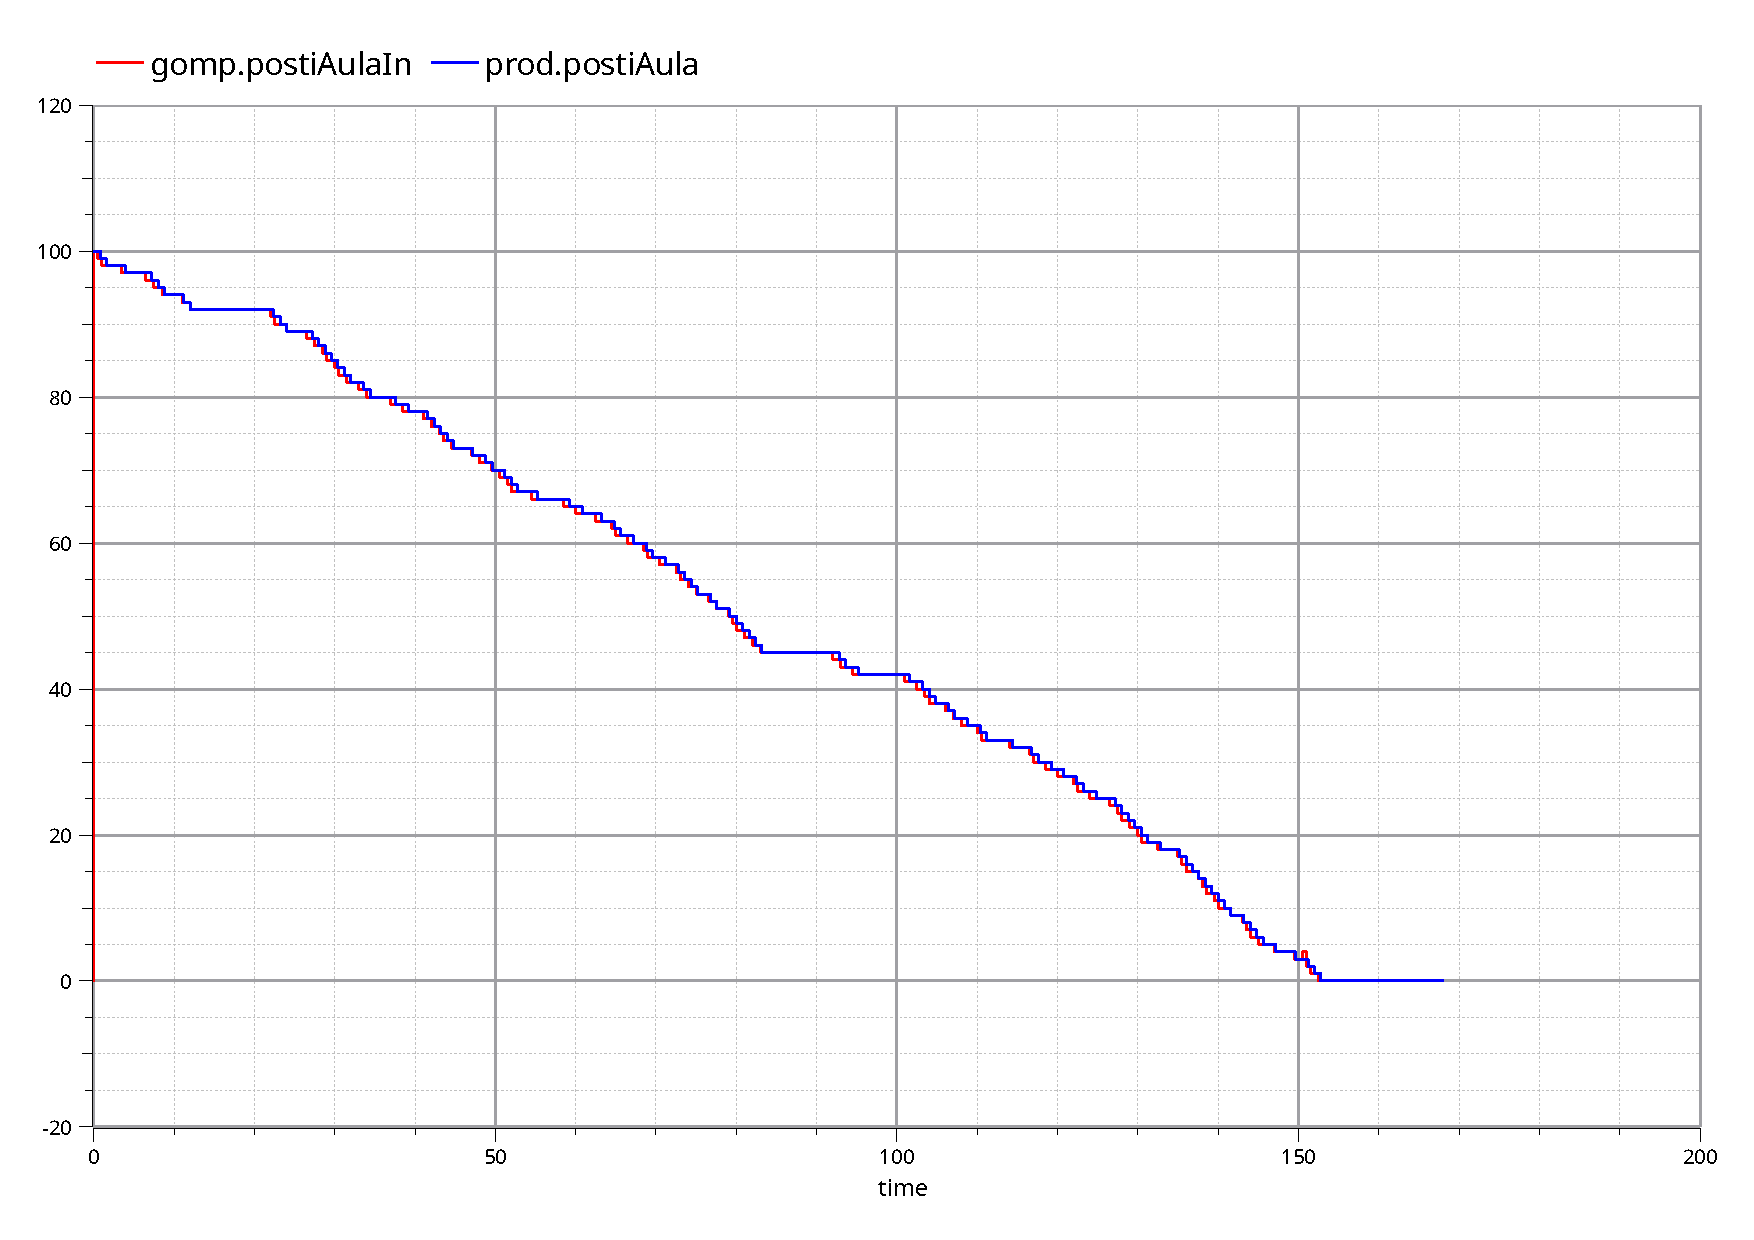
\includegraphics[width=1 \textwidth]{Figure/studente solo prenotazioni.pdf}
    \caption{Grafico che mostra l’andamento dei posti nell’aula nel caso estremo in cui siano presenti solo prenotazioni, è utile notare  l’ultima parte del grafico che rimane costante al valore 0 fino alla fine della simulazione.} \label{figura: solo prenotazioni}
\end{center}
\end{figure}

Nel caso opposto (ovvero con solo cancellazioni) a quello mostrato in figura si otterrà una linea costante.\\

Un altro caso estremo che si può considerare è quello in cui Prodigit è sempre non raggiungibile e quindi non si ha la possibilità di effettuare nessuna azione, ciò è visibile dal grafico nella figura ~\ref{figura:prodigit down}, in cui è evidente che i posti dell’aula rimangono  costanti al valore iniziale.

\begin{figure}[htp]
\begin{center}
  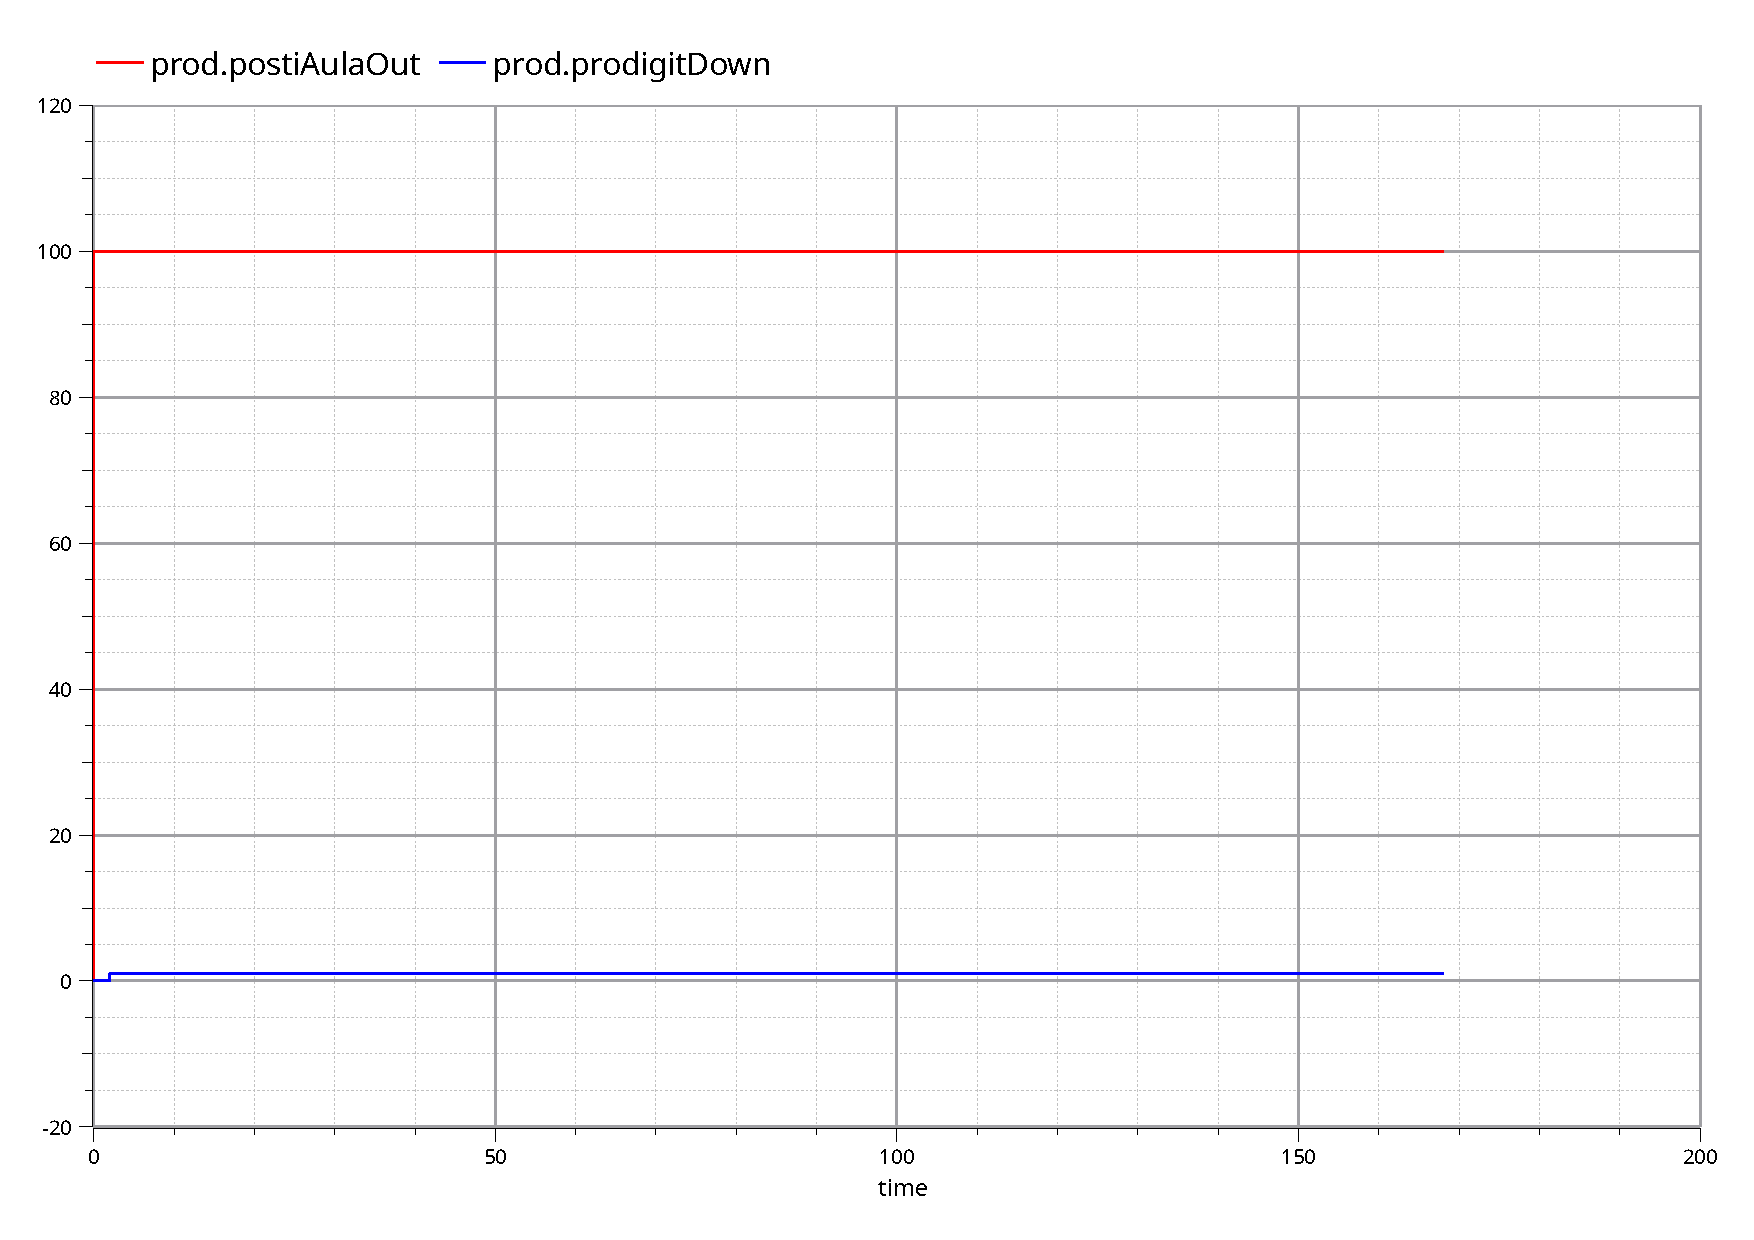
\includegraphics[width=1 \textwidth]{Figure/posti prod down.pdf}
    \caption{Grafico che rappresenta il caso in cui Prodigit è costantemente down, l’andamento della variazione dei posti  è costante al valore iniziale.}\label{figura:prodigit down}
\end{center}
\end{figure}


\chapter*{Architettura di sistema}

\par Prima di analizzare il sistema bisogna specificare alcune scelte fatte nel corso dello sviluppo:
\begin{enumerate}
\item Nel sistema  è presente un’unica aula con capienza pari a 100, ma è facilmente ampliabile con più aule seguendo lo stesso ragionamento.
\item Il tempo del sistema usa come unità  di misura T=1, che viene fatto corrispondere ad un’ora, quindi tutto il tempo è calibrato su questa unità.
\item Per rimanere concorde con le specifiche il sistema viene eseguito per una settimana ovvero 168 (${24}\cdot{7}$) unità di tempo (colpi di clock).
\item Le probabilità vengono calcolate con seed casuali, utilizzando la libreria \textbf{Modelica.Math.Random} di Mdelica.
\end{enumerate}

\par Di seguito viene spiegata l’implementazione dei vari oggetti del sistema e il loro ruolo:
\begin{description}
\item [Aula:] rappresenta l’oggetto aula ed è definita tramite un blocco nel file \textit{aula.mo}. Non ha nessun input ed il suo unico scopo è quello di variare il suo stato: ha una probabilità $\frac{9}{10}$ di essere agibile ad ogni colpo di clock, i cambiamenti vengono valutati ogni 15 minuti (ovvero T=0.25), l’informazione sul suo stato viene passata al Gomp che a sua volta la passerà a Prodigit, nel caso in cui verifica che l’aula sia agibile darà la possibilità allo studente di effettuare una prenotazione o una cancellazione su di essa.
\item [Studente:] rappresenta l’utente del sistema definito tramite un blocco nel file \textit{studente.mo}, non ha input ed ha la possibilità di richiedere una prenotazione o una cancellazine comunicando tramite una variabile di output con il sistema Prodigit, la probabilità con cui fare richiesta è di un $\frac{1}{2}$, rappresentando la suddivisione in turni delle matricole, il blocco effettua questo controllo ogni 12 minuti ovvero con T pari a 0.20.
\item [Gomp:] rappresenta il sistema esterno dell’università e contiene varie informazioni, definito tramite un blocco nel file \textit{gomp.mo}, ottiene in input lo stato dell’aula, può variare il suo stato da \textit{operativo} (con probabilità $\frac{9}{10}$) a \textit{non operativo} e viceversa. Contiene inoltre  la capienza iniziale dell’aula che verrà aggiornata periodicamente da Prodigit.
\item [Prodigit:] definito tramite un blocco nel file \textit{prodigit.mo}, come prima cosa controlla lo stato del sistema Gomp decidendo di conseguenza se essere operativo o meno, nel caso in cui sia disponibile controlla che siano verificate tutte le condizioni per effettuare una prenotazione (con probabilità $\frac{7}{10}$ ) oppure una cancellazione con probabilità  $\frac{3}{10}$, ciò viene fatto chiamando le funzioni appropriate, infine calcola la media dei fallimenti tramite una funzione dedicata in modo tale da passare questa informazione al monitor non funzionale.

\item [Funzioni:] il sistema usufruisce di varie funzioni: per effettuare una prenotazione, andando a decrementare i posti disponibili all’interno dell’aula, una cancellazione, aumentando i posti disponibili e per il calcolo della media dei fallimenti.

\item [Monitor:] tramite delle variabili prese in input verificano se il sistema riespetta i requisiti.

\item [System:] questo blocco ha l’unico scopo di mettere in comunicazione i vari blocchi collegando gli input con i giusti output.
\end{description}
\chapter*{Requisiti di sistema}
Durante lo sviluppo mi sono preoccupato di rispettare i seguenti requisiti, di cui due funzionali ed uno non funzionale:
\par Il rpimo requisito funzionale è quello della \textbf{Safety}, ovvero preoccuparsi di non fare mai \textit{overbooking} (cioè, prenotare per un aula un numero di studenti superiore alla capienza covid dell’aula). Questo viene rispettato grazie ad una condizione di controllo (all’interno del blocco \textbf{Prodigit}) che non permette di prenotare se nell’aula non ci sono più posti disponibili.
\par L’altro requisito funzionale è quello della \textbf{Liveness}, finché ci sono posti disponibili per gli eventi, le richieste di prenotazione non vengono rifiutate. Anche in questo caso, come il requisito precedente, viene gestito all’interno del sistema \textbf{Prodigit} che  non permette di cancellare una prenotazione se non ci sono prenotazioni attive, ovvero se il numero di posti disponibili è uguale alla capienza originale dell’aula.\\
 Questi requisiti vengono verificati dal monitor funzionale (nel file \textit{monitorFun.mo})  tramite una variabile booleana inizializzata a \textit{false} che  non appena il monitor rileva la violazione del requisito mette la variabile \textit{true}.\newline

\par Il requisito non funzionale del sistema è il seguente: si vuole che Prodigit sia down al più per il 80\% del tempo per cui il Gomp è down. Quindi, ad esempio, se il Gomp è down per un ora al giorno, prodigit potrà essere down al più per 48 minuti al giorno.\\ 
Viene verificato all’interno del monitor non funzionale nel file \textit{monitorNotFun}, conoscendo il numero di volte in cui Gomp è down ed il numero di volte in cui Prodigit è down ne calcola la media tramite cui controlla se il requisito è rispettato.
 
\chapter*{Risultati sperimentali}
Vengono ora riportate alcune immagini che raffigurano vari output del sistema, ottenute eseguendo il file \textit{run.mos}.

\begin{figure}[htp]
\begin{center}
  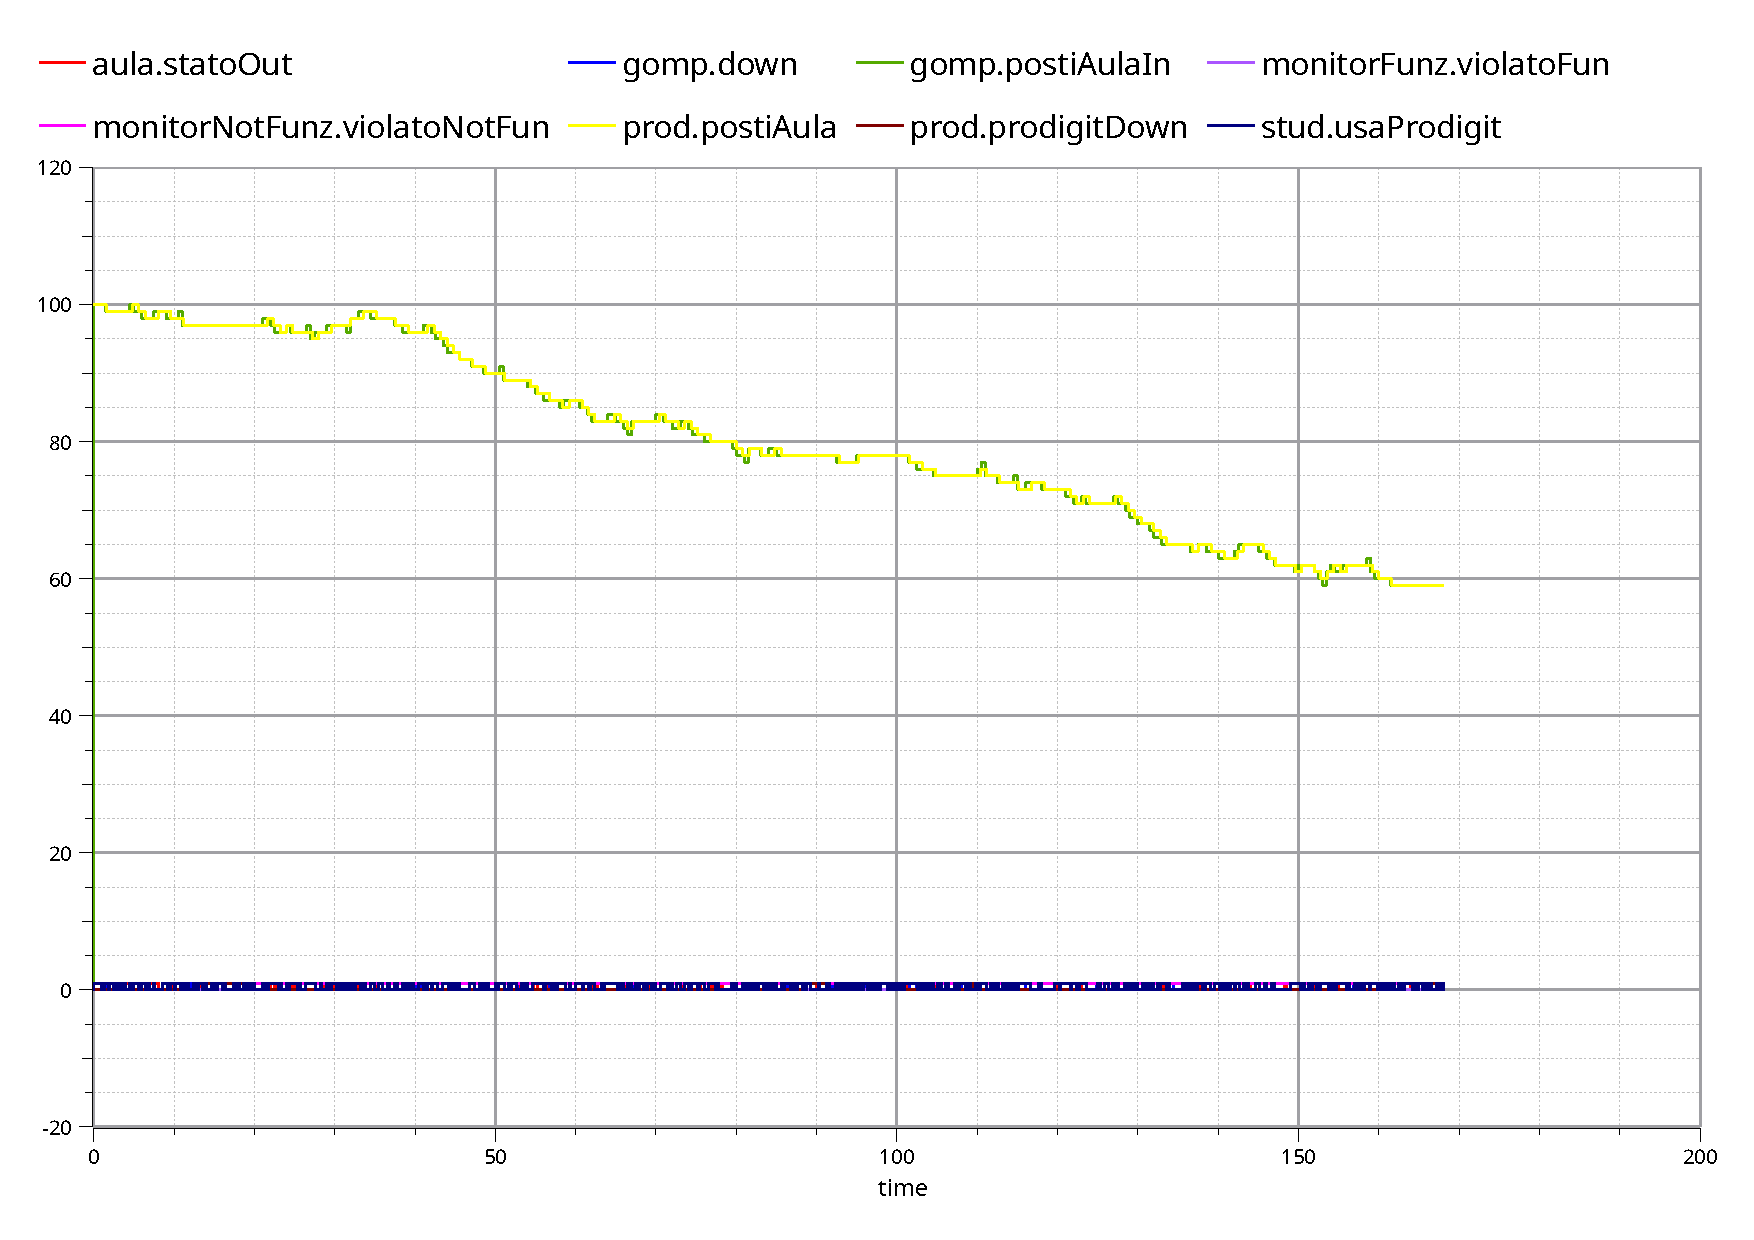
\includegraphics[width=1 \textwidth]{Figure/plot finale.pdf}
    \caption{Immagine che mostra tutti gli output del sistema, oltre all’andamento della capienza dell’aula si possono notare i monitor e gli stati  delle varie componenti.} \label{figura: finale}
\end{center}
\end{figure}

Nella figura ~\ref{figura: prodigit down} viene riportato il grafico dei posti in relazione allo stato del sistema Prodigit, come si può notare quando lo stato del sistema è su 1 ( quindi è non disponibile) allora non ci sono incrementi o decrementi sulla capienza, lo stesso avviene considerando lo stato dell’aula.
Si può anche notare la linea arancione che indica che il monitor funzionale non viene mai violato.\\

Tramite i due script Python \textit{verify.py} e \textit{synth.py} si ha la possibilità di eseguire il programma (senza ottenere la stampa) un gran numero di volte con diversi parametri verificando ogni volta la robustezza del sistema controllando il comportamento del monitor.\\
Il primo esegue il sistema 100, 1000, 10000 volte,  il suo intento è quello di verificare il requisito funzionale, per fare ciò ad ogni iterazione assegna una variabile casuale tra 4 possibili (una di default, due agli estremi ed una a metà) controllando quindi il risultato del mointor sul valore assegnato. Il \textit{synth.py} invece si occupa del requisito non funzionale eseguendo il sistema 100 o 1000 volte, anche in questo caso seleziona con la setssa idea 4 possibili variabili.\\



\begin{figure}[htp]
\begin{center}
  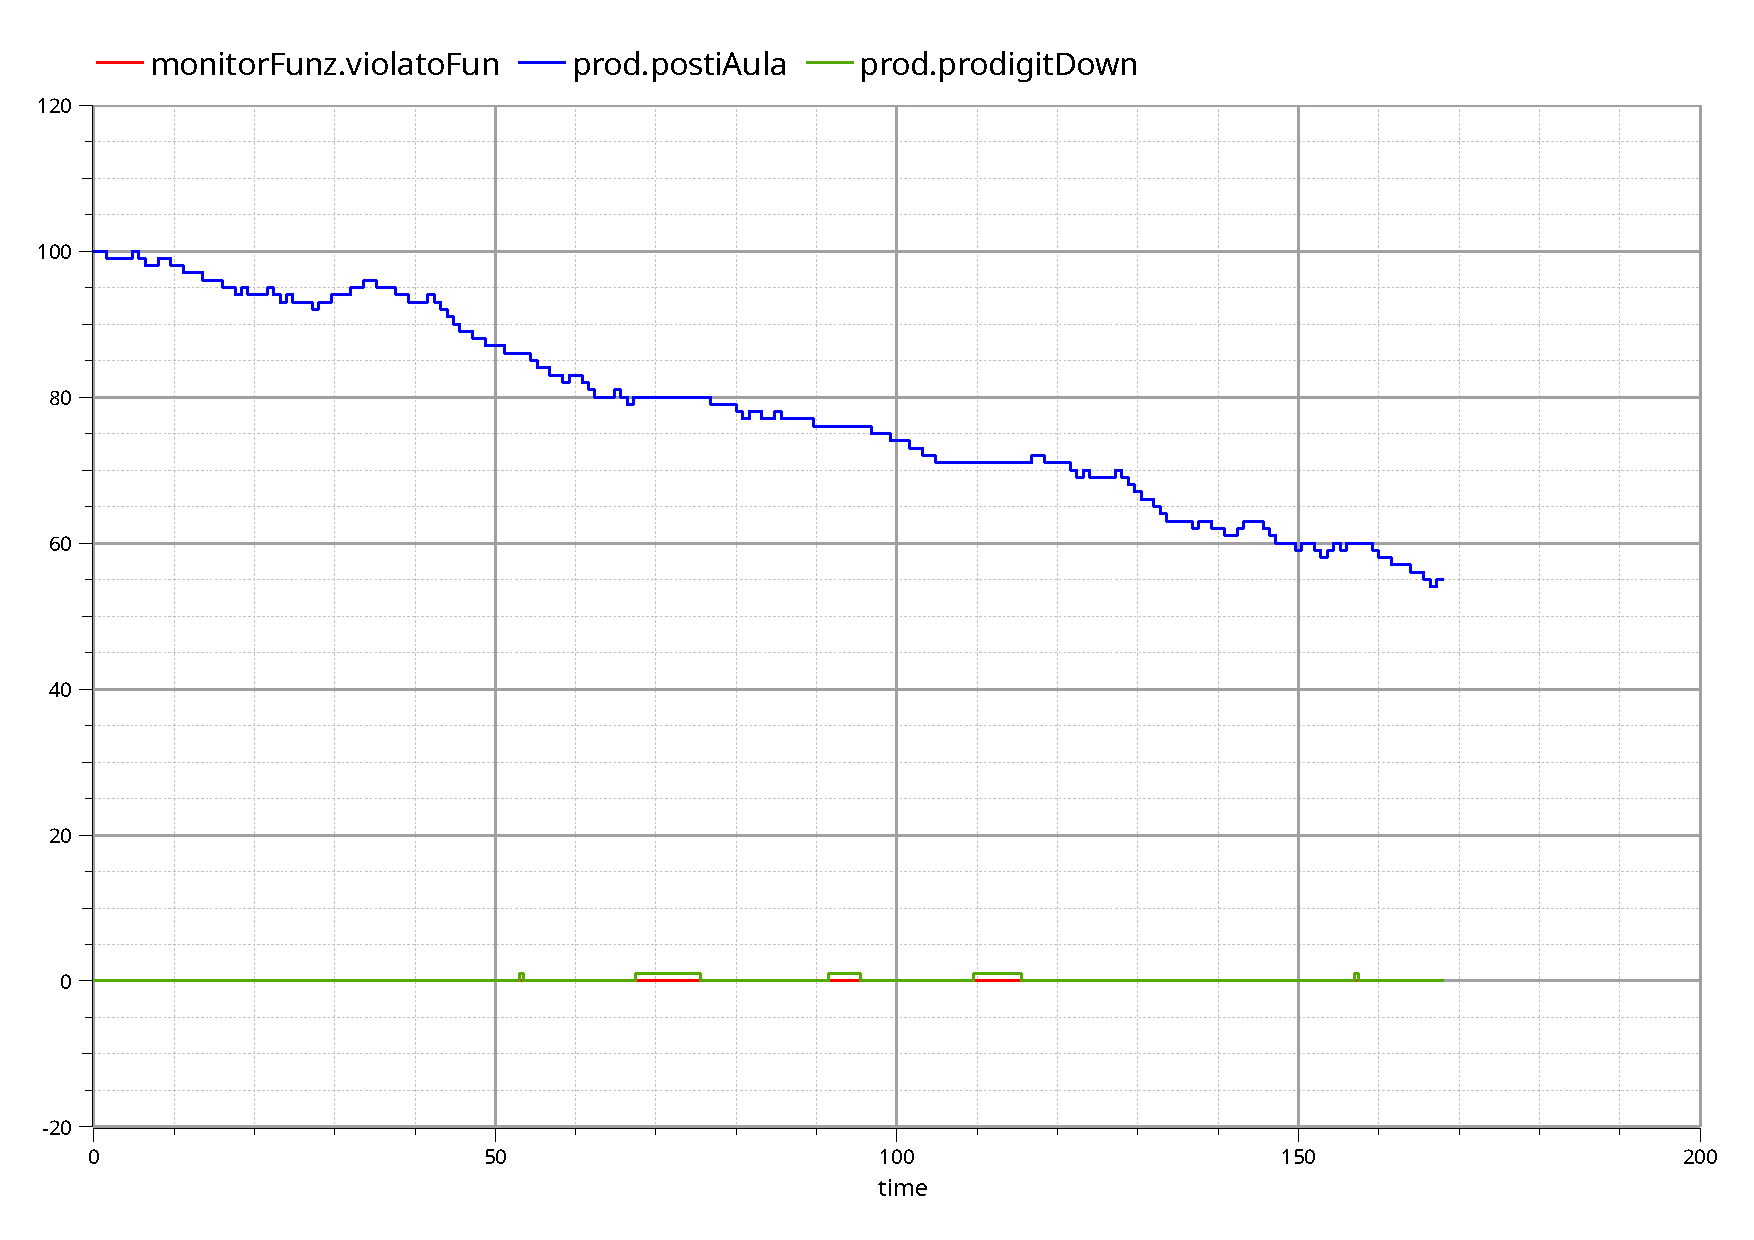
\includegraphics[width=1 \textwidth]{Figure/prodigit down.pdf}
    \caption{Grafico che mostra la relazione tra lo stato del sistema Prodigit e la capienza dell’aula.} \label{figura: prodigit down}
\end{center}
\end{figure}

La figura  ~\ref{figura: prodigit e gomp} mostra invece la relazione tra lo stato di Prodigit e quello di Gomp.\\

\begin{figure}[htp]
\begin{center}
  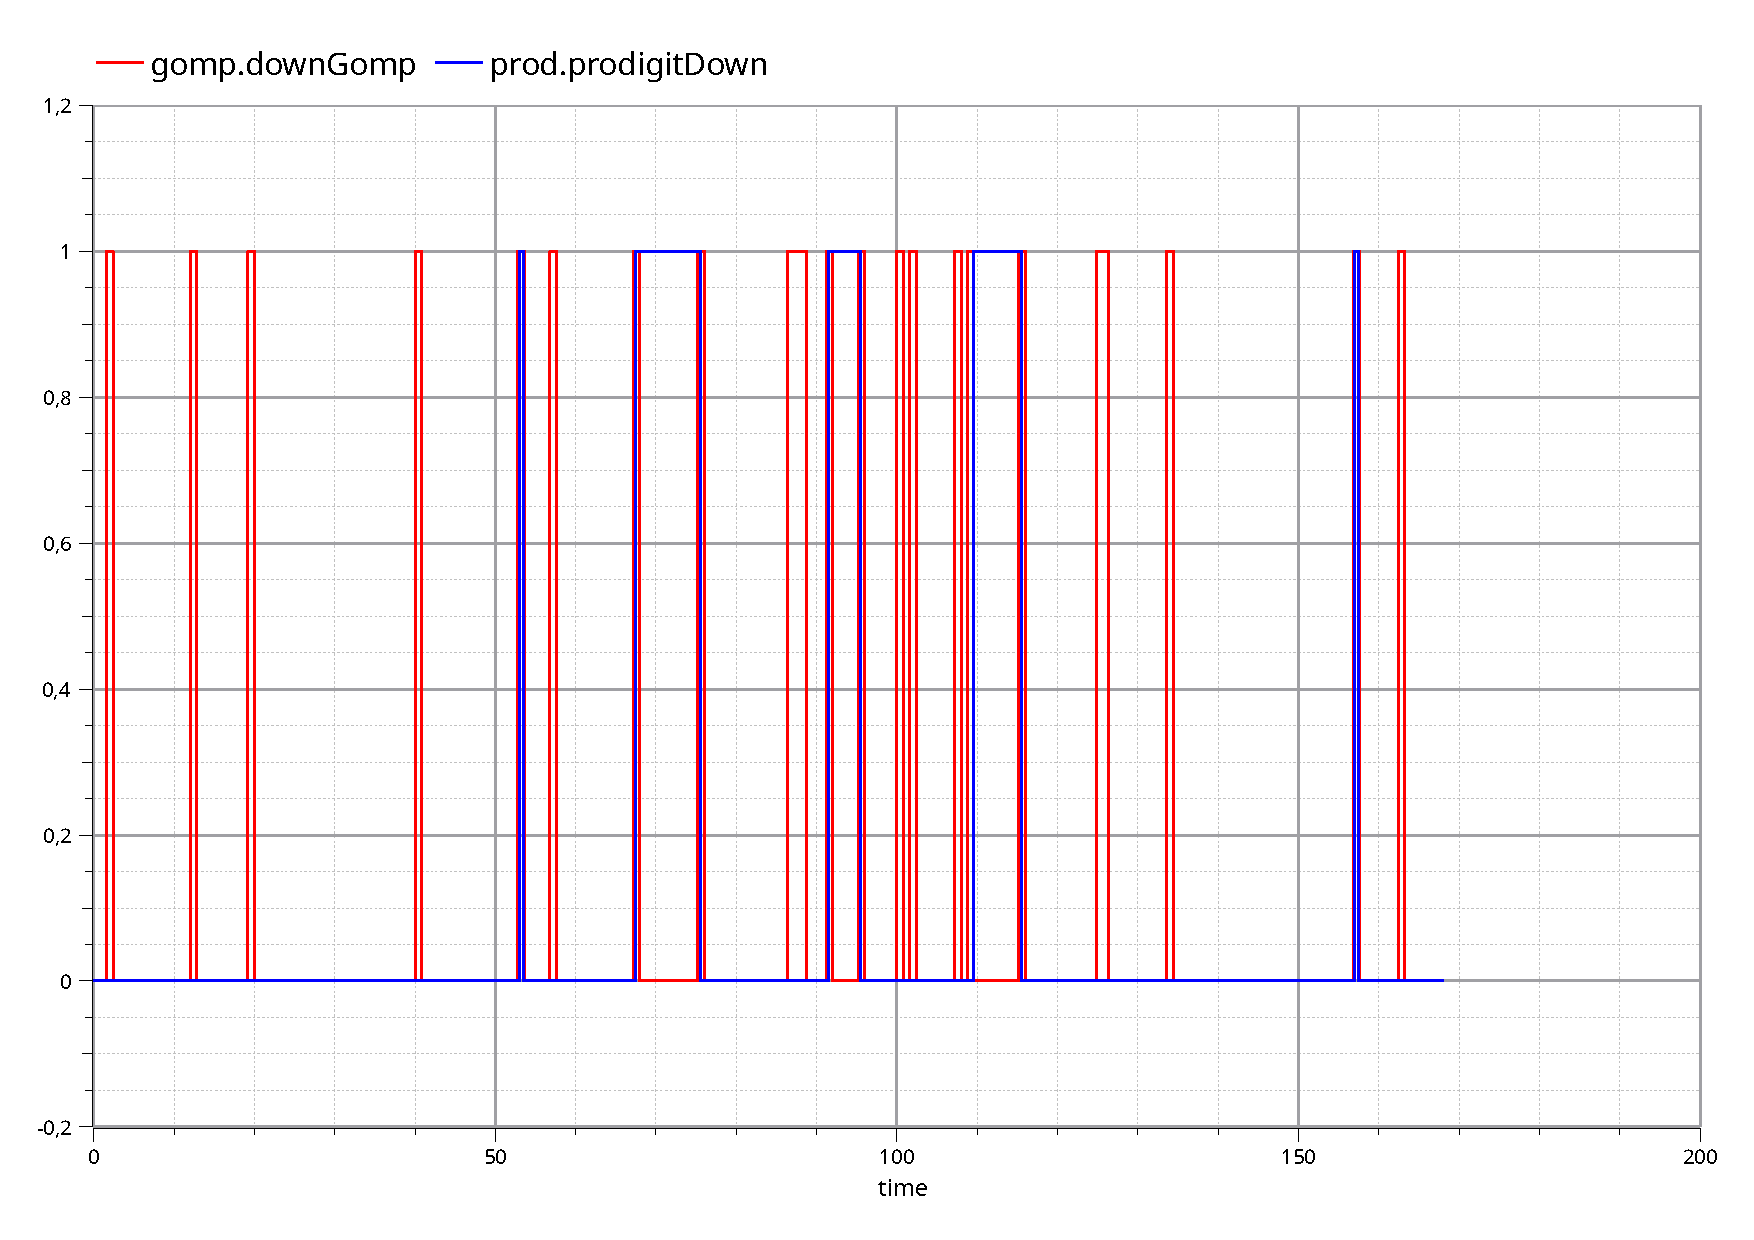
\includegraphics[width=1 \textwidth]{Figure/prod e gomp down.pdf}
    \caption{Grafico che rappresenta lo stato di Prodigit (in blu) e quello di Gomp (in arancione).}\label{figura: prodigit e gomp} 
\end{center}
\end{figure}




\end{document}